\documentclass[a4paper,oneside,11pt]{book}

% Package yang diperlukan
\usepackage{graphicx}
\usepackage{titling}
\usepackage{geometry}
\usepackage{listings}
\usepackage{xcolor}
\usepackage{float}
\usepackage{hyperref}
\usepackage{indentfirst}
\usepackage{caption}
\usepackage{array}
\usepackage{enumitem}
\usepackage[htt]{hyphenat}
\setlength{\emergencystretch}{3em}

% Pengaturan margin
\geometry{
    left=3cm,
    right=2.5cm,
    top=3cm,
    bottom=3cm
}

% Pengaturan untuk kode
\definecolor{codegreen}{rgb}{0,0.6,0}
\definecolor{codegray}{rgb}{0.5,0.5,0.5}
\definecolor{codepurple}{rgb}{0.58,0,0.82}
\definecolor{backcolour}{rgb}{0.95,0.95,0.92}

\lstdefinestyle{htmlstyle}{
    backgroundcolor=\color{backcolour},
    commentstyle=\color{codegreen},
    keywordstyle=\color{codepurple},
    numberstyle=\tiny\color{codegray},
    stringstyle=\color{codegreen},
    basicstyle=\ttfamily\footnotesize,
    breakatwhitespace=false,
    breaklines=true,
    captionpos=b,
    keepspaces=true,
    numbers=left,
    numbersep=5pt,
    showspaces=false,
    showstringspaces=false,
    showtabs=false,
    tabsize=2,
    frame=single
}

\title{Laporan Tugas \\ Konstruksi dan Evolusi Perangkat Lunak \\
Pertemuan 11 \\
Penerapan Monitoring dengan Prometheus dan Grafana}
\author{Nama Mahasiswa: Brilian Fatih Wicaksono (24/535871/SV/24320)}
\date{\today}

\begin{document}

% Halaman judul
\begin{titlingpage}
\begin{center}
\vspace{4cm}
\begin{huge}
\textbf{\thetitle} \\
\end{huge}
\vspace{2cm}

\includegraphics[height=8cm]{lambang ugm.png}\\
\begin{Large}
\vspace{4cm}
\theauthor\\
Kelas BB \\
\end{Large}
\begin{large}
Dosen Pengampu: Galih Malela Damaraji, S.Pd., M.Eng.\\
\end{large}
\vspace{2cm}
\thedate
\end{center}
\end{titlingpage}

% Daftar Isi
\tableofcontents
\newpage

\chapter{Tujuan Praktikum}
\begin{enumerate}[leftmargin=*]
    \item Menyusun satu berkas Compose yang menjalankan Prometheus, Grafana, cAdvisor, dan node-exporter bersama aplikasi Hunian Pegawai, dengan versi image terkunci serta volume data Prometheus dan Grafana.
    \item Memastikan seluruh target pada halaman \texttt{/targets} Prometheus berstatus \texttt{UP} dan membuktikannya melalui tangkapan layar.
    \item Membuat satu dashboard Grafana terprovisioning berisi minimal empat panel yang menjawab pertanyaan nyata tentang aplikasi ini, lengkap dengan satuan dan ambang.
    \item Menulis satu aturan alarm dengan \texttt{for:} dan anotasi tindakan pertama, lalu membuktikan alarm berubah dari \texttt{inactive} menjadi \texttt{FIRING} ketika layanan dimatikan.
    \item Menerapkan keamanan dasar dengan mengganti kredensial bawaan Grafana dan menjelaskan alasan penggantian tersebut.
\end{enumerate}

\chapter{Dasar Teori}

\section{Model Pull dan Push}
Pemantauan dapat dibagi menjadi dua pola pengumpulan data. Pada model \emph{push}, aplikasi atau agen mengirim metrik ke server pemantauan. Pada model \emph{pull}, server pemantauan yang aktif mengambil metrik dari endpoint milik target secara berkala. Prometheus menggunakan model pull: setiap \texttt{scrape\_interval}, Prometheus menghubungi endpoint \texttt{/metrics} pada target, membaca teks berformat khusus, lalu menyimpannya sebagai time series. Model ini membuat status target dapat dinilai langsung dari keberhasilan pengambilan data; jika endpoint tidak dapat dihubungi, Prometheus mencatat \texttt{up = 0}. Model pull juga memudahkan penemuan target dan pengujian endpoint secara manual dengan alat sederhana seperti \texttt{curl}.

\section{Peran Prometheus dan Grafana}
Prometheus adalah basis data time series sekaligus mesin evaluasi aturan. Ia menyimpan sampel metrik, menjalankan bahasa kueri PromQL, dan mengevaluasi aturan alarm. Grafana bukan penyimpan metrik; ia adalah lapisan visualisasi dan eksplorasi yang membaca data dari datasource seperti Prometheus. Pemisahan ini penting: Prometheus bertanggung jawab atas pengumpulan, penyimpanan, dan peringatan, sedangkan Grafana bertanggung jawab atas penyajian dashboard, panel, dan pengalaman pengguna. Dashboard yang baik bukan sekadar kumpulan grafik, melainkan kumpulan pertanyaan operasional yang dijawab oleh data.

\section{Jenis Metrik, PromQL, dan \texttt{rate()}}
Prometheus mengenal beberapa jenis metrik utama. \emph{Counter} hanya bertambah dan cocok untuk jumlah permintaan atau total waktu CPU. \emph{Gauge} dapat naik dan turun, misalnya pemakaian memori. \emph{Histogram} dan \emph{summary} digunakan untuk distribusi nilai seperti durasi permintaan. PromQL menyediakan operator pemilihan label, agregasi \texttt{sum by}, serta fungsi laju. Counter tidak boleh dibaca mentah karena nilainya terus naik; ia harus dibungkus fungsi seperti \texttt{rate(http\_requests\_total[5m])} yang menghitung laju per detik dalam jendela lima menit. Jendela waktu harus lebih besar dari interval scrape agar hasil tidak kosong atau berkedip.

\section{Bahaya Kardinalitas Label}
Setiap kombinasi label menghasilkan time series baru. Label yang bernilai hampir unik, misalnya ID pengguna, ID transaksi, atau path URL mentah, dapat meledakkan jumlah time series dan membebani memori Prometheus. Karena itu label rute pada aplikasi ini memakai pola rute Laravel, bukan path sebenarnya. Permintaan yang tidak cocok dengan rute mana pun diberi label tetap \texttt{tidak\_cocok}. Dengan cara ini jumlah kombinasi label tetap terkendali walaupun ada banyak ID berbeda.

\section{Alerting}
Aturan alarm di Prometheus terdiri atas ekspresi, durasi \texttt{for:}, label, dan anotasi. Ekspresi menentukan kondisi bermasalah, misalnya \texttt{up\{job="aplikasi"\} == 0}. Durasi \texttt{for:} mencegah alarm berbunyi karena lonjakan sesaat; kondisi harus benar terus-menerus selama durasi tersebut. Label seperti \texttt{severity: kritis} membantu pengelompokan dan routing. Anotasi \texttt{summary} menjelaskan masalah, sedangkan anotasi \texttt{action} memberi tahu tindakan pertama yang harus dilakukan operator. Alarm yang baik dapat dipahami tanpa membuka dashboard terlebih dahulu.

\section{Keamanan Dasar}
Monitoring menyimpan informasi operasional dan memberi akses ke sistem. Kredensial bawaan seperti \texttt{admin/admin} berbahaya karena mudah ditebak dan sering menjadi sasaran pemindaian otomatis. Password harus dibuat acak, disimpan di luar repositori, dan diberikan melalui variabel lingkungan atau secret manager. Port administratif sebaiknya hanya terbuka di loopback atau jaringan internal. Pendaftaran pengguna mandiri juga perlu dimatikan bila tidak diperlukan. Prinsip least privilege dan pemisahan rahasia dari kode adalah fondasi keamanan dasar.

\chapter{Implementasi dan Hasil}

\section{Susunan Compose dan Target}
Stack monitoring dijalankan bersama aplikasi melalui dua berkas Compose: \texttt{docker-compose.yml} untuk aplikasi dan \texttt{compose.monitoring.yaml} untuk layanan monitoring. Perintah yang dipakai adalah:

\begin{lstlisting}[language={},style=htmlstyle]
docker compose -f docker-compose.yml -f compose.monitoring.yaml up -d --build
\end{lstlisting}

Kedua berkas berada pada satu project Compose sehingga seluruh container memakai network default yang sama. Nama service dapat langsung menjadi hostname, misalnya \texttt{backend:8000}, \texttt{cadvisor:8080}, dan \texttt{prometheus:9090}. Versi image dikunci secara eksplisit:
\begin{itemize}[leftmargin=*]
    \item \texttt{prom/prometheus:v2.53.0}
    \item \texttt{grafana/grafana:11.1.0}
    \item \texttt{gcr.io/cadvisor/cadvisor:v0.49.1}
    \item \texttt{prom/node-exporter:v1.8.1}
    \item \texttt{redis:7.4.4-alpine}
    \item \texttt{node:20.15.1-alpine}
\end{itemize}
Volume bernama \texttt{prom-data}, \texttt{grafana-data}, dan \texttt{redis-data} menjaga data tetap ada ketika container dibuat ulang.

\begin{lstlisting}[language={},style=htmlstyle]
services:
  prometheus:
    image: prom/prometheus:v2.53.0
    volumes:
      - ./monitoring/prometheus.yml:/etc/prometheus/prometheus.yml:ro
      - ./monitoring/alerts.yml:/etc/prometheus/alerts.yml:ro
      - prom-data:/prometheus
    ports:
      - "127.0.0.1:9090:9090"

  grafana:
    image: grafana/grafana:11.1.0
    environment:
      GF_SECURITY_ADMIN_PASSWORD: ${GRAFANA_PASS:?isi GRAFANA_PASS di .env}
      GF_USERS_ALLOW_SIGN_UP: "false"
    volumes:
      - grafana-data:/var/lib/grafana
      - ./monitoring/grafana/provisioning:/etc/grafana/provisioning:ro
    ports:
      - "127.0.0.1:3000:3000"
\end{lstlisting}

Port Prometheus dan Grafana hanya diikat ke \texttt{127.0.0.1}. cAdvisor, node-exporter, Redis, dan exporter tidak dipublikasikan ke host. Konfigurasi scrape memakai empat job dan interval 15 detik:

\begin{lstlisting}[language={},style=htmlstyle]
global:
  scrape_interval: 15s
  evaluation_interval: 15s

rule_files:
  - /etc/prometheus/alerts.yml

scrape_configs:
  - job_name: prometheus
    static_configs:
      - targets: ["localhost:9090"]
  - job_name: container
    static_configs:
      - targets: ["cadvisor:8080", "docker-exporter:9101"]
  - job_name: server
    static_configs:
      - targets: ["node-exporter:9100"]
  - job_name: aplikasi
    metrics_path: /metrics
    static_configs:
      - targets: ["backend:8000"]
\end{lstlisting}

Hasil pemeriksaan \texttt{promtool check config} dan \texttt{promtool check rules} berhasil tanpa kesalahan. Setelah menunggu lebih dari 30 detik, halaman \texttt{/targets} menampilkan seluruh target berstatus \texttt{UP}, seperti terlihat pada Gambar \ref{fig:targets}. Terdapat lima endpoint karena job \texttt{container} memiliki dua target, yaitu cAdvisor dan exporter statistik Docker.

\begin{figure}[htbp]
    \centering
    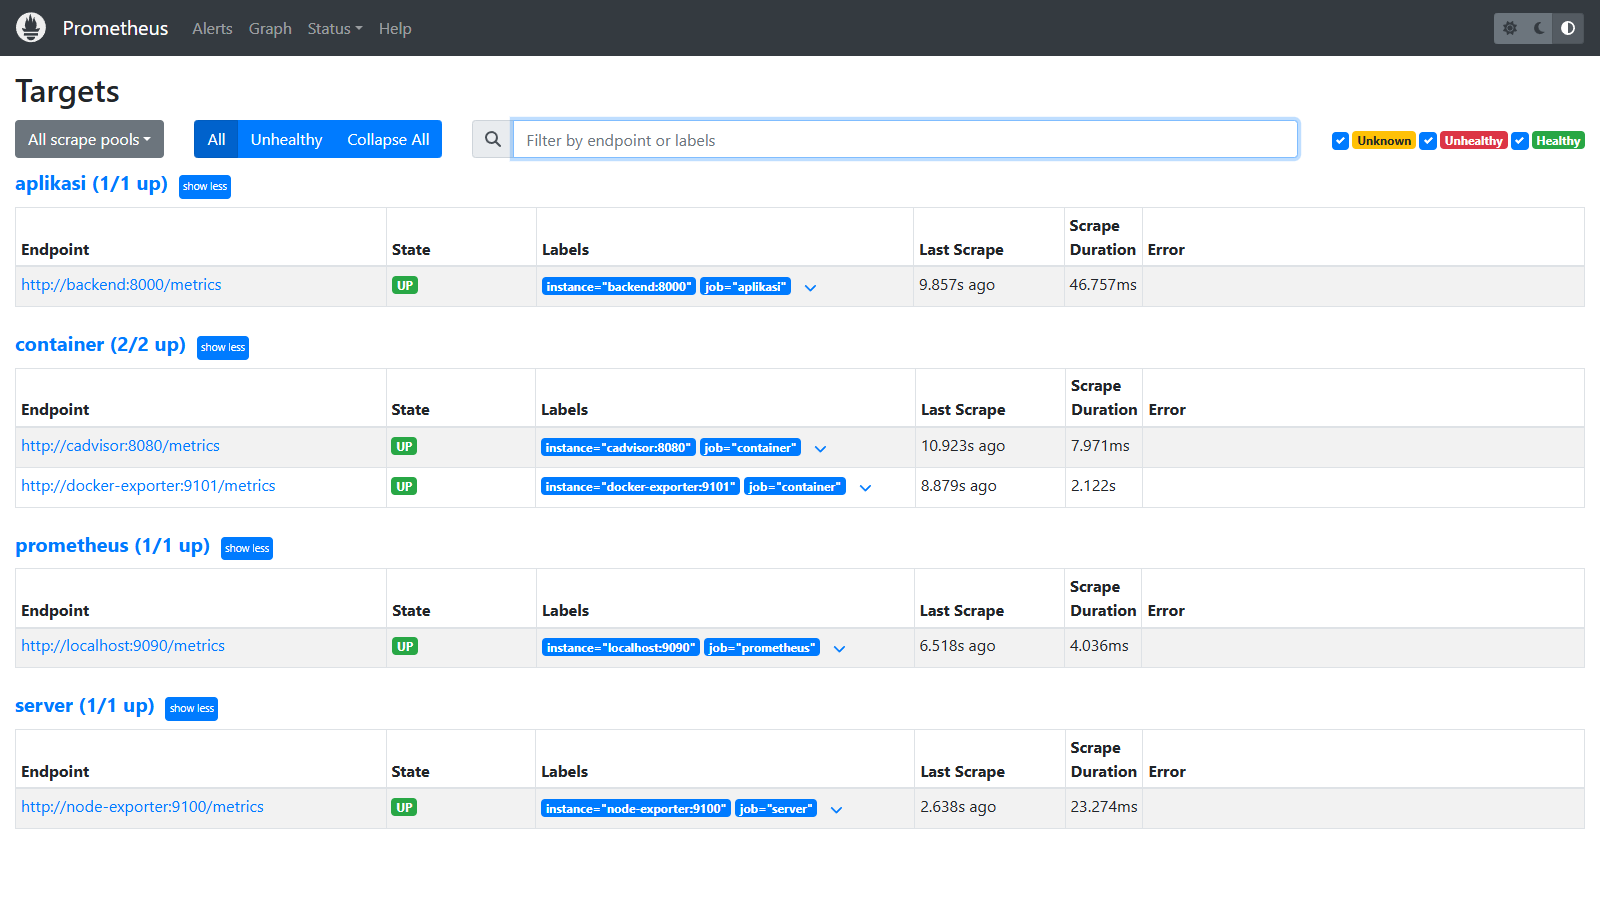
\includegraphics[width=\textwidth,keepaspectratio]{gambar/01-targets.png}
    \caption{Halaman \texttt{/targets} Prometheus. Lima endpoint dari empat job berstatus \texttt{UP} dan tidak ada target \texttt{DOWN}.}
    \label{fig:targets}
\end{figure}

Pada Docker Desktop dengan Docker Engine 29 dan containerd image store, cAdvisor v0.49.1 gagal membaca metadata layer Docker. Log cAdvisor menunjukkan pesan \texttt{failed to identify the read-write layer ID} sehingga hanya metrik agregat yang muncul. Konfigurasi \texttt{cgroup: host}, mount \texttt{/var/run}, dan \texttt{/sys} sudah dicoba, tetapi label \texttt{name} tetap tidak tersedia. Sebagai solusi yang jujur dan tetap terukur, ditambahkan service \texttt{docker-exporter} yang membaca Docker API melalui \texttt{/var/run/docker.sock} dan mengekspos \texttt{container\_cpu\_usage\_seconds\_total} serta \texttt{container\_memory\_usage\_bytes} dengan label \texttt{name}. cAdvisor tetap berjalan dan target-nya tetap \texttt{UP}. Selain itu, mount \texttt{rslave} untuk node-exporter tidak didukung Docker Desktop sehingga diturunkan menjadi \texttt{/:/host:ro}. Basis image backend juga dipindahkan ke \texttt{dunglas/frankenphp:php8.3-bookworm} karena repositori Debian trixie menolak verifikasi tanda tangan pada jam sistem pengujian.

\section{Metrik Aplikasi}
Aplikasi Laravel dilayani oleh FrankenPHP pada port 8000. Karena FrankenPHP menggunakan proses PHP bertipe ZTS, APCu tidak dipilih. Penyimpanan metrik memakai Redis melalui paket \texttt{promphp/prometheus\_client\_php} versi \texttt{\^2.15} dan adapter \texttt{Prometheus\textbackslash{}Storage\textbackslash{}Redis}. Dengan demikian nilai counter bertahan antar-request dan tetap terbaca oleh proses scraping Prometheus. Redis dijalankan sebagai service pendukung dan hanya dapat diakses dari network Compose.

Endpoint \texttt{GET /metrics} didaftarkan langsung pada bootstrap aplikasi agar tidak melewati session web. Middleware \texttt{RecordHttpMetrics} menghitung \texttt{http\_requests\_total} dengan label \texttt{method}, \texttt{route}, dan \texttt{status}. Label \texttt{route} diambil dari pola rute Laravel, misalnya \texttt{api/housing-units/\{housing\_unit\}}, bukan dari path mentah. Permintaan tanpa rute cocok, termasuk 404, memakai label tetap \texttt{tidak\_cocok}. Endpoint \texttt{/metrics} dan \texttt{/api/health} dikecualikan agar pengambilan metrik tidak menghitung dirinya sendiri.

\begin{lstlisting}[language=PHP,style=htmlstyle]
private function record(Request $request, int $status): void
{
    $path = trim($request->path(), '/');

    if ($path === 'metrics' || $path === 'api/health') {
        return;
    }

    $route = $request->route();
    $routeLabel = $route !== null ? $route->uri() : 'tidak_cocok';

    $this->registry
        ->getOrRegisterCounter(
            '',
            'http_requests_total',
            'Jumlah permintaan HTTP yang diterima aplikasi.',
            ['method', 'route', 'status']
        )
        ->inc([$request->method(), $routeLabel, (string) $status]);
}
\end{lstlisting}

Traffic nyata dibangkitkan dari host menggunakan \texttt{curl.exe} selama lebih dari 25 menit, dari pukul 22.29.55 sampai 22.54.54. Setiap siklus mengirim enam permintaan: login dengan kredensial salah (401), \texttt{/api/user}, \texttt{/api/housing-units}, \texttt{/api/maintenance-tickets}, \texttt{/api/placements}, dan satu URL yang tidak ada (404). Total ada 740 siklus atau lebih dari 4.000 permintaan. Log mentah disimpan pada \texttt{laporan/log/06-traffic.txt}. Setelah beberapa siklus, \texttt{/metrics} menampilkan counter untuk setiap kombinasi method, route, dan status. Prometheus kemudian membaca metrik tersebut dan seluruh kueri dashboard mengembalikan data.

\section{Dashboard Grafana}
Datasource Prometheus dan dashboard diprovisioning melalui berkas YAML serta JSON, bukan melalui klik manual. Datasource memakai UID tetap \texttt{prometheus} dan URL internal \texttt{http://prometheus:9090}. Provider dashboard bertipe file membaca folder \texttt{/etc/grafana/provisioning/dashboards}. Dashboard berjudul \emph{Monitoring Aplikasi Hunian Pegawai} memakai UID tetap \texttt{kepl-p11-hunian}. Lima panel disusun untuk menjawab pertanyaan, bukan sekadar menampilkan metrik:

\begin{enumerate}[leftmargin=*]
    \item \emph{Apakah semua layanan hidup?} menampilkan \texttt{up} per job dengan value mapping 1 = UP (hijau) dan 0 = DOWN (merah).
    \item \emph{Berapa persen permintaan yang gagal?} memakai rasio 5xx terhadap seluruh permintaan, unit \texttt{percentunit}, ambang merah 0,05.
    \item \emph{Berapa banyak permintaan masuk per detik?} memakai laju permintaan lima menit, unit \texttt{reqps}.
    \item \emph{Berapa CPU yang dipakai tiap container?} memakai laju CPU per container, unit \texttt{percentunit}.
    \item \emph{Berapa memori yang dipakai tiap container?} memakai gauge memori per container, unit \texttt{bytes} (IEC).
\end{enumerate}

Kueri PromQL yang dipakai kelima panel adalah:

\begin{lstlisting}[language={},style=htmlstyle]
up
(sum(rate(http_requests_total{status=~"5.."}[5m])) or vector(0))
  / sum(rate(http_requests_total[5m]))
sum(rate(http_requests_total[5m]))
sum by (name) (rate(container_cpu_usage_seconds_total{name!=""}[5m]))
container_memory_usage_bytes{name!=""}
\end{lstlisting}

Panel status ditempatkan di kiri atas, diikuti rasio gagal dan permintaan per detik pada baris yang sama. Baris kedua memuat CPU dan memori per container. Setiap panel memiliki deskripsi, satuan, dan garis ambang. Ketika dashboard dibuka dengan rentang 15 menit terakhir, tidak ada teks \emph{No data} dan tidak ada panel error. Hasilnya terlihat pada Gambar \ref{fig:dashboard}. Query panel CPU juga dapat diperiksa langsung melalui mode edit seperti pada Gambar \ref{fig:panelquery}.

\begin{figure}[htbp]
    \centering
    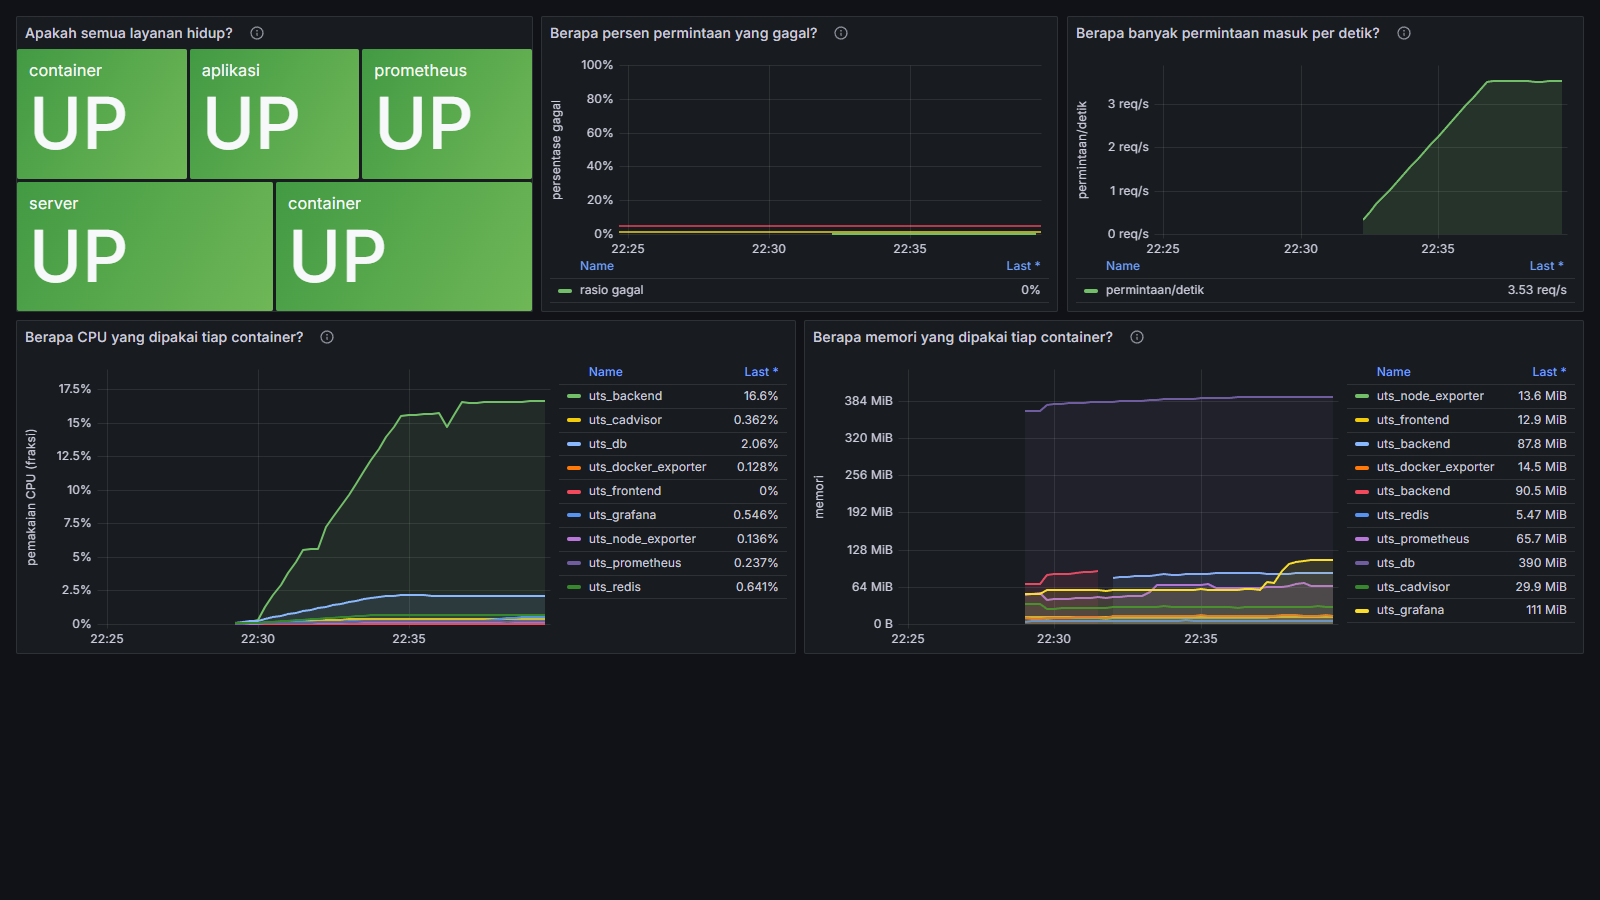
\includegraphics[width=\textwidth,keepaspectratio]{gambar/02-dashboard.png}
    \caption{Dashboard lengkap dengan lima panel pertanyaan. Semua layanan UP, permintaan sekitar 3,53 per detik, dan rasio gagal 0 persen.}
    \label{fig:dashboard}
\end{figure}

\begin{figure}[htbp]
    \centering
    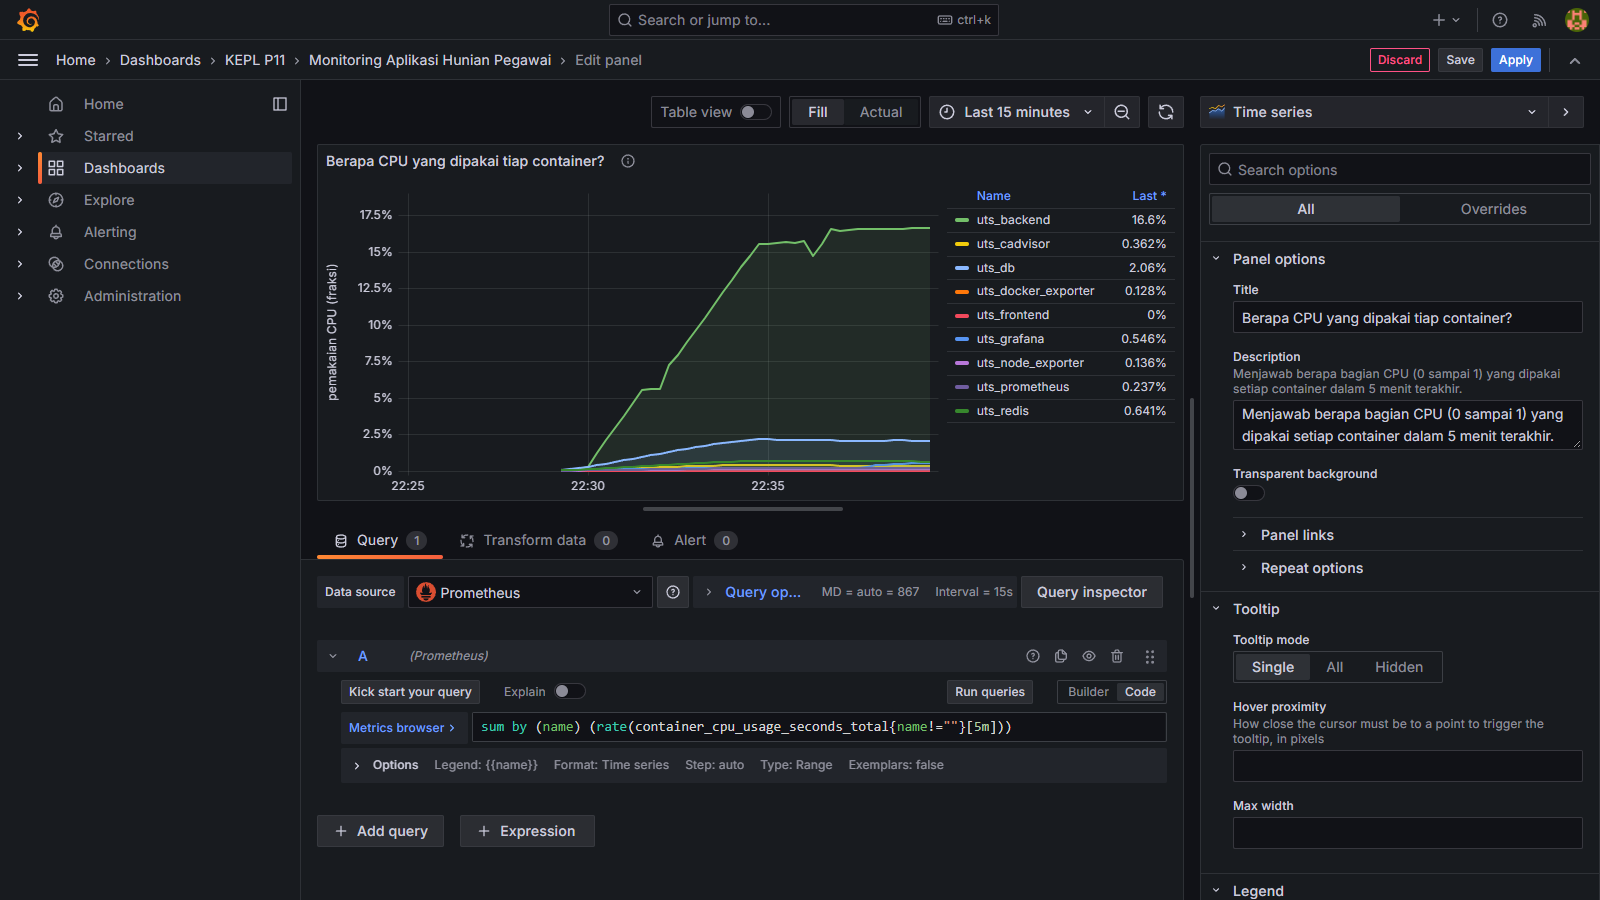
\includegraphics[width=\textwidth,keepaspectratio]{gambar/03-panel-query.png}
    \caption{Mode edit panel CPU memperlihatkan kueri laju CPU per container beserta legenda nama container.}
    \label{fig:panelquery}
\end{figure}

\section{Alarm}
Satu aturan alarm ditulis pada \texttt{monitoring/alerts.yml}. Aturan ini memakai ekspresi \texttt{up\{job="aplikasi"\} == 0}, durasi \texttt{for: 1m}, label \texttt{severity: kritis}, serta dua anotasi. Anotasi \texttt{summary} menyatakan bahwa aplikasi tidak dapat ditarik. Anotasi \texttt{action} menyebut tindakan pertama yang konkret, yaitu menjalankan \texttt{docker compose ps} lalu \texttt{docker compose logs backend}. Kedua perintah memakai nama service sebenarnya sehingga dapat langsung dieksekusi.

\begin{lstlisting}[language={},style=htmlstyle]
groups:
  - name: aplikasi-hunian
    rules:
      - alert: LayananMati
        expr: up{job="aplikasi"} == 0
        for: 1m
        labels:
          severity: kritis
        annotations:
          summary: "Aplikasi Hunian Pegawai tidak bisa ditarik oleh Prometheus."
          action: "Jalankan `docker compose ps`, lalu `docker compose logs backend` untuk memeriksa penyebab container berhenti."
\end{lstlisting}

Sebelum pengujian, halaman \texttt{/alerts} menunjukkan \texttt{LayananMati} dalam keadaan \emph{Inactive} dengan 0 active, seperti pada Gambar \ref{fig:alertinactive}. Pengujian dilakukan dengan menghentikan container backend pada pukul 22.40.36. Ekspresi mulai bernilai benar pada pukul 22.40.50, kemudian status terlihat \emph{pending} pada polling berikutnya. Setelah melewati durasi satu menit, aturan berubah menjadi \emph{firing} dan terdeteksi pada pukul 22.42.08. Total waktu dari container berhenti sampai alarm FIRING adalah 92 detik, sedangkan durasi dari status pending sampai firing sekitar 61 detik. Nilai ini sesuai dengan \texttt{for: 1m} ditambah jeda evaluasi dan scrape.

\begin{figure}[htbp]
    \centering
    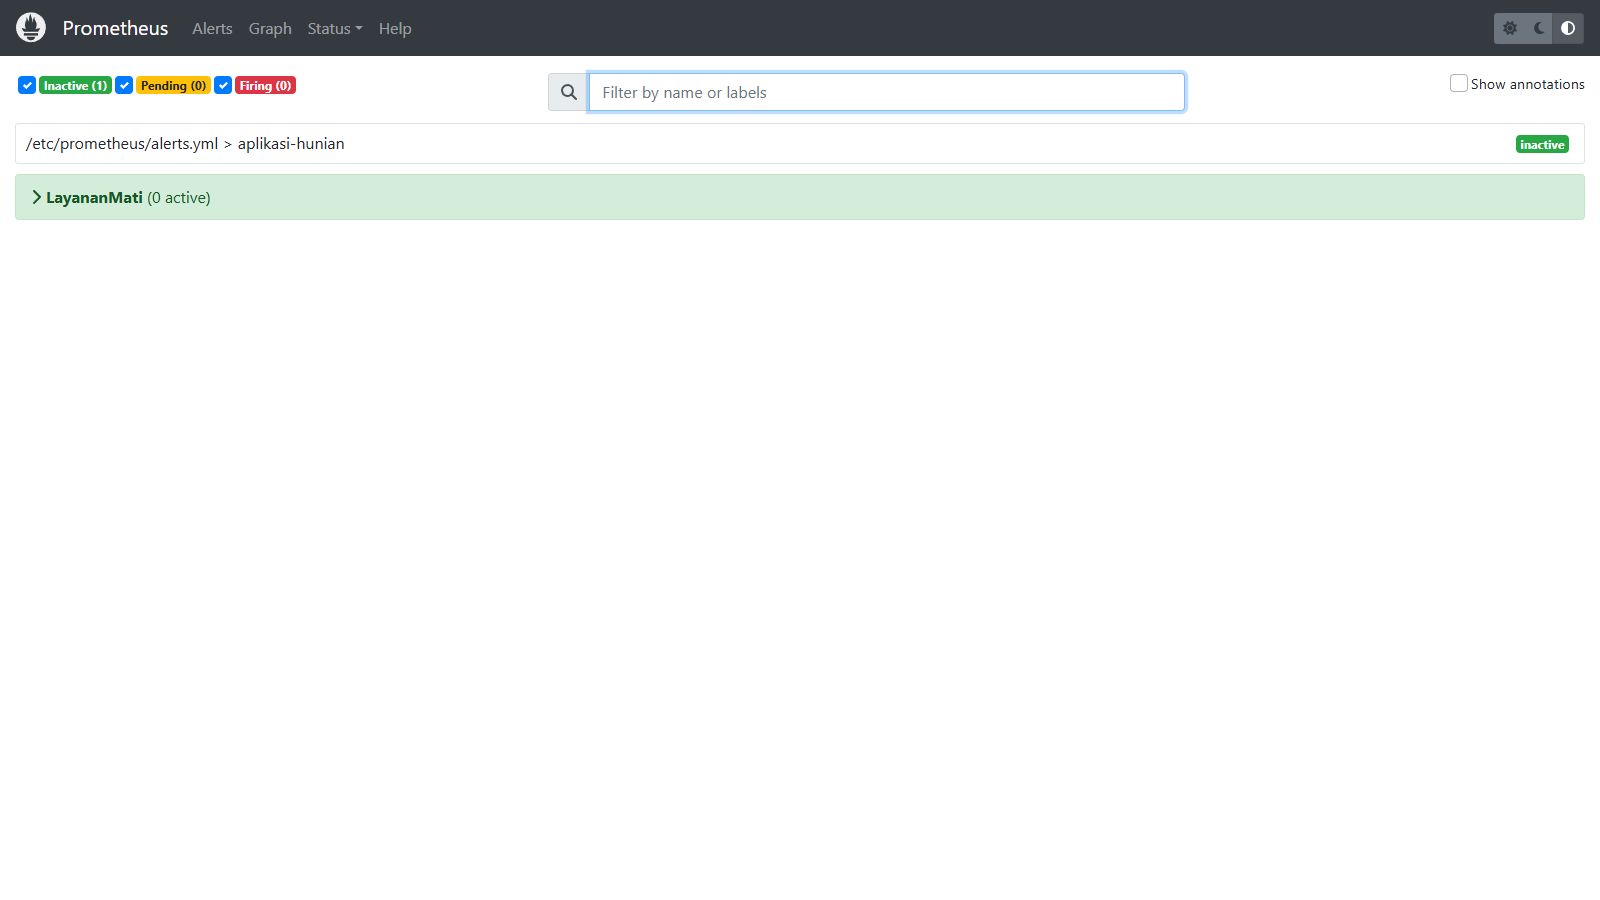
\includegraphics[width=\textwidth,keepaspectratio,trim=0 650 0 0,clip]{gambar/04-alert-inactive.png}
    \caption{Halaman \texttt{/alerts} sebelum pengujian. Aturan \texttt{LayananMati} berstatus \emph{Inactive} dengan 0 active.}
    \label{fig:alertinactive}
\end{figure}

Saat FIRING, halaman \texttt{/alerts} menampilkan label \texttt{alertname}, \texttt{instance}, \texttt{job}, \texttt{severity=kritis}, serta anotasi \texttt{summary} dan \texttt{action}. Bukti tersebut ditunjukkan pada Gambar \ref{fig:alertfiring}. Halaman \texttt{/targets} juga menampilkan target aplikasi berstatus \texttt{DOWN} dengan pesan error DNS karena container backend sudah berhenti (Gambar \ref{fig:targetdown}). Dashboard ikut menampilkan panel status merah bertuliskan DOWN untuk job aplikasi (Gambar \ref{fig:dashboarddown}).

\begin{figure}[htbp]
    \centering
    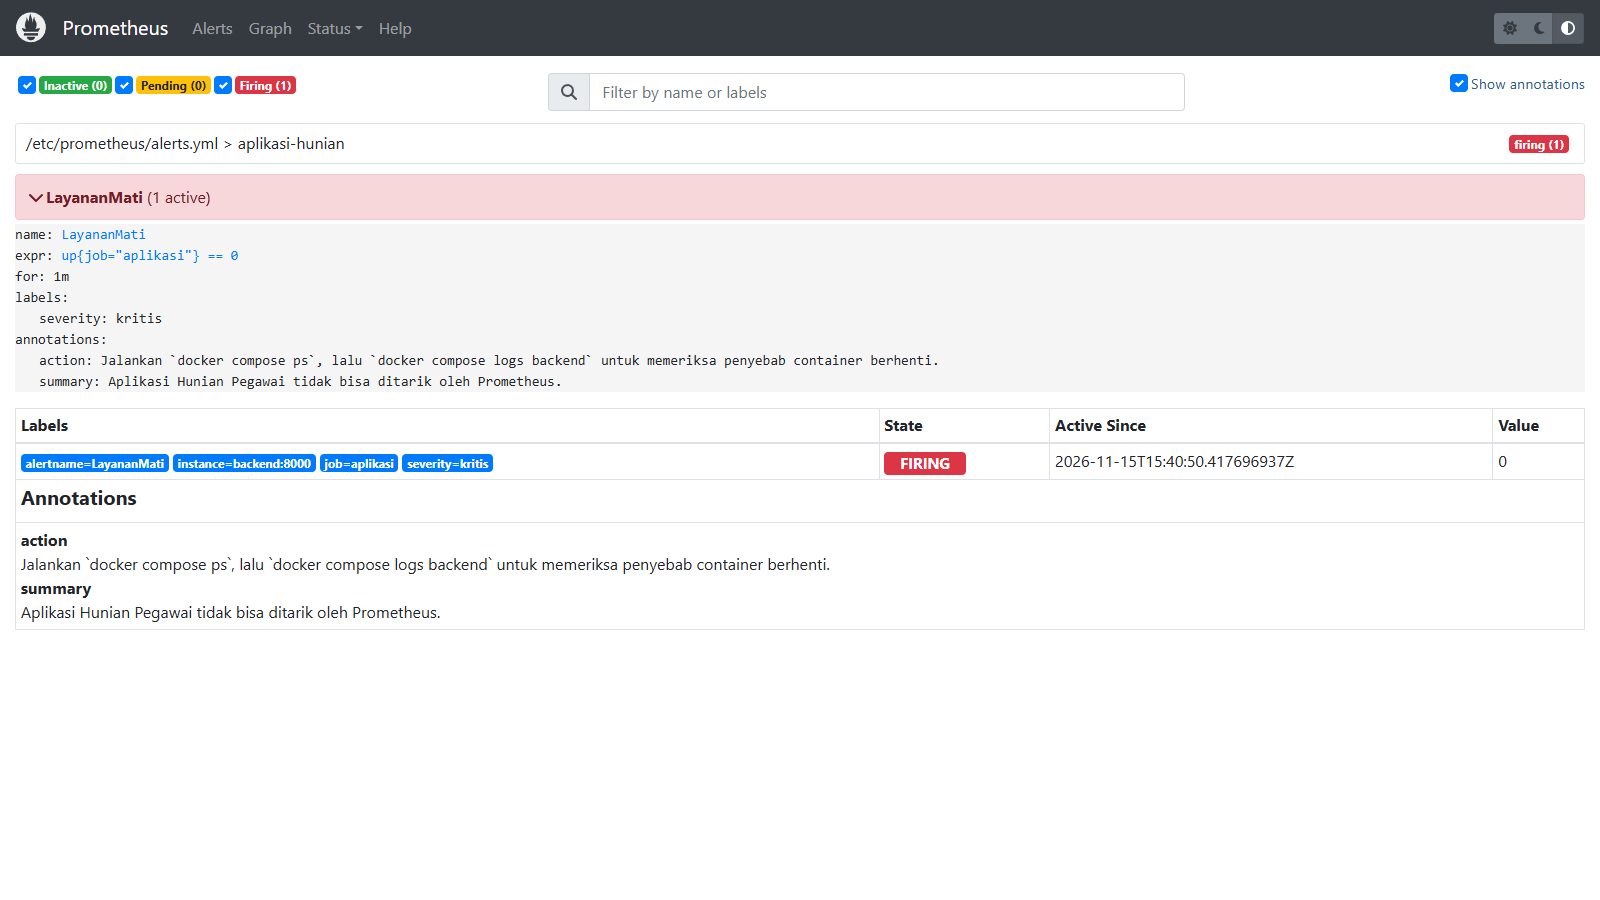
\includegraphics[width=\textwidth,keepaspectratio,trim=0 240 0 0,clip]{gambar/05-alert-firing.png}
    \caption{Alarm \texttt{LayananMati} berstatus FIRING. Anotasi \texttt{action} menyebut perintah pertama yang harus dijalankan operator.}
    \label{fig:alertfiring}
\end{figure}

\begin{figure}[htbp]
    \centering
    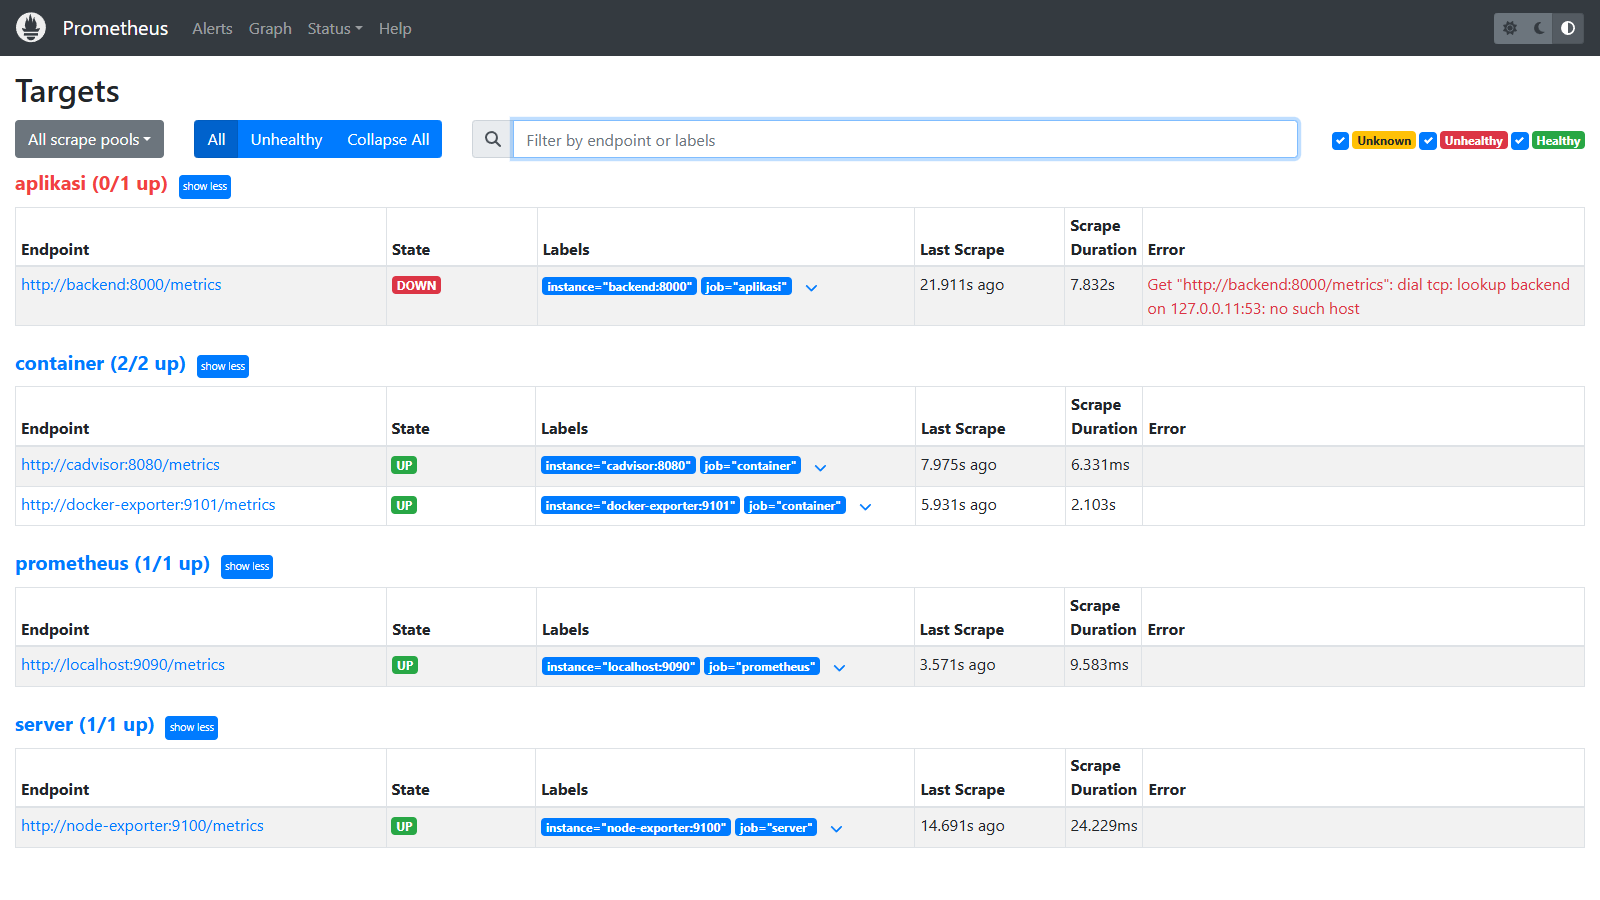
\includegraphics[width=\textwidth,keepaspectratio]{gambar/06-target-down.png}
    \caption{Halaman \texttt{/targets} saat backend dimatikan; target aplikasi berubah menjadi \texttt{DOWN}.}
    \label{fig:targetdown}
\end{figure}

\begin{figure}[htbp]
    \centering
    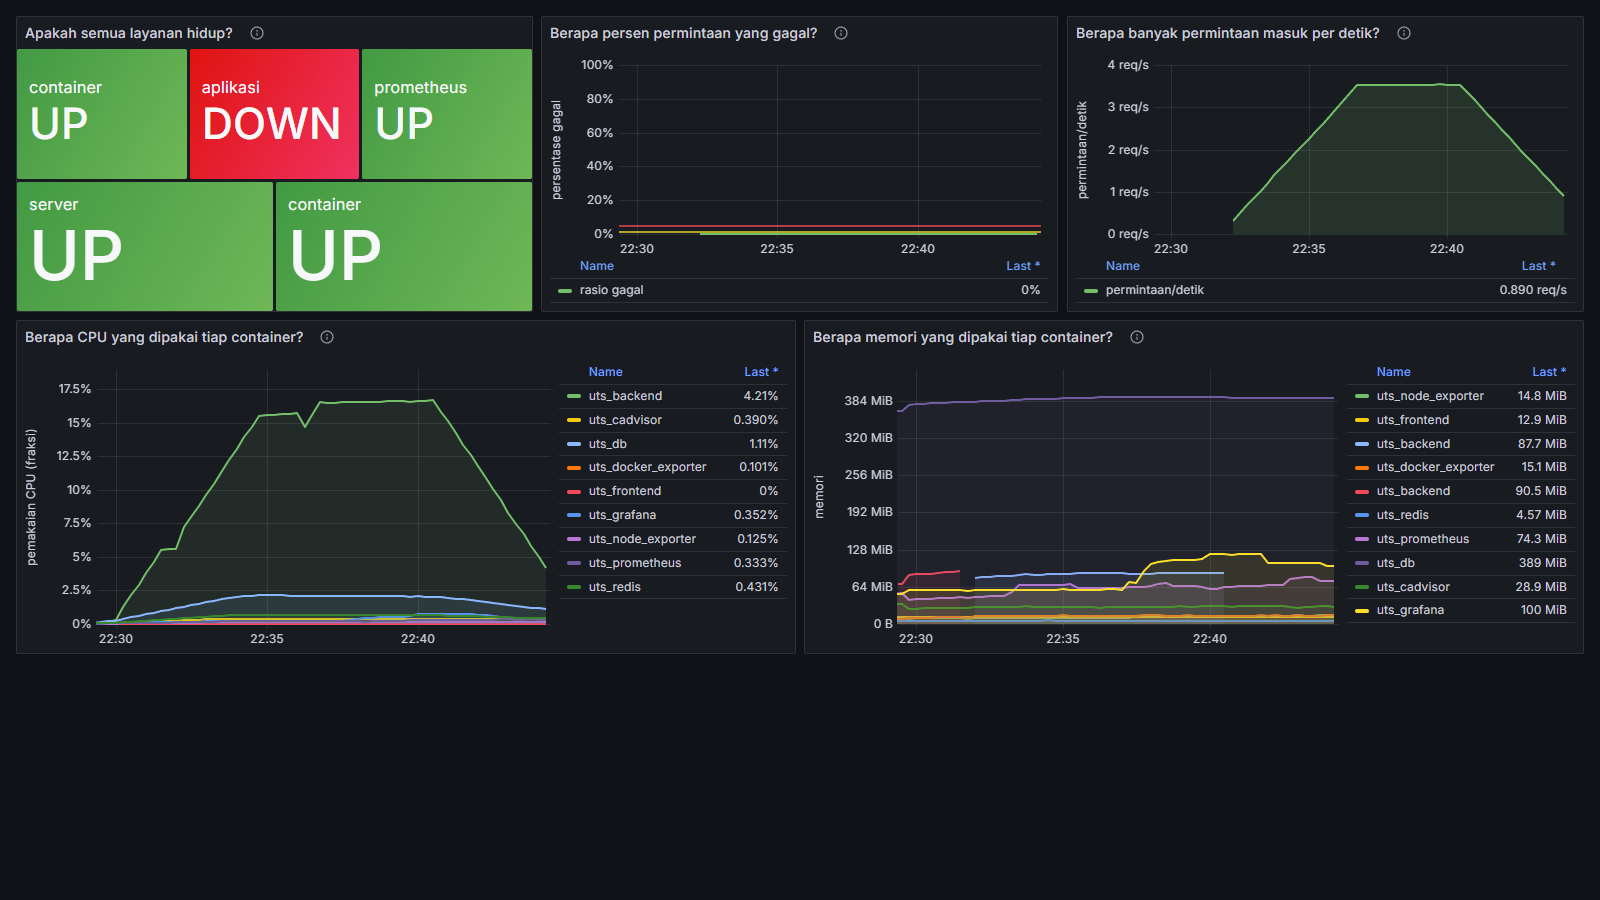
\includegraphics[width=\textwidth,keepaspectratio]{gambar/07-dashboard-down.png}
    \caption{Dashboard saat layanan mati. Panel status menampilkan aplikasi DOWN berwarna merah, sementara layanan monitoring lain tetap UP.}
    \label{fig:dashboarddown}
\end{figure}

Setelah backend dinyalakan kembali, target aplikasi kembali \texttt{UP} dalam 16 detik. Alarm kembali tidak aktif setelah 47 detik, yaitu setelah satu siklus evaluasi berikutnya. Rincian waktu pengujian disimpan pada \texttt{laporan/log/07-alarm-test.txt}.

\section{Keamanan}
Password admin Grafana tidak ditulis di berkas yang di-commit. Nilai \texttt{GRAFANA\_PASS} dibaca dari \texttt{.env} di root repo, sedangkan \texttt{.env.example} hanya berisi placeholder. Berkas \texttt{.env} sudah masuk \texttt{.gitignore} dan diperiksa dengan \texttt{git check-ignore}. Pendaftaran pengguna mandiri dimatikan melalui \texttt{GF\_USERS\_ALLOW\_SIGN\_UP=false}. Port Grafana dan Prometheus hanya terikat ke \texttt{127.0.0.1}, sehingga tidak terbuka ke jaringan luar. cAdvisor, node-exporter, Redis, dan exporter tidak mempublikasikan port sama sekali.

Kredensial bawaan \texttt{admin/admin} berbahaya karena merupakan nilai yang diketahui publik dan sering dicoba oleh pemindai otomatis. Jika dibiarkan, siapa pun yang dapat menjangkau port Grafana berpotensi membaca data operasional, mengubah dashboard, atau mematikan alarm. Oleh karena itu password acak dibuat dan dimasukkan melalui variabel lingkungan. Untuk membuktikan penggantian berhasil, percobaan login dengan \texttt{admin/admin} ditolak dengan pesan \emph{Invalid username or password}, seperti pada Gambar \ref{fig:loginditolak}. Password asli tidak pernah ditampilkan pada tangkapan layar.

\begin{figure}[H]
    \centering
    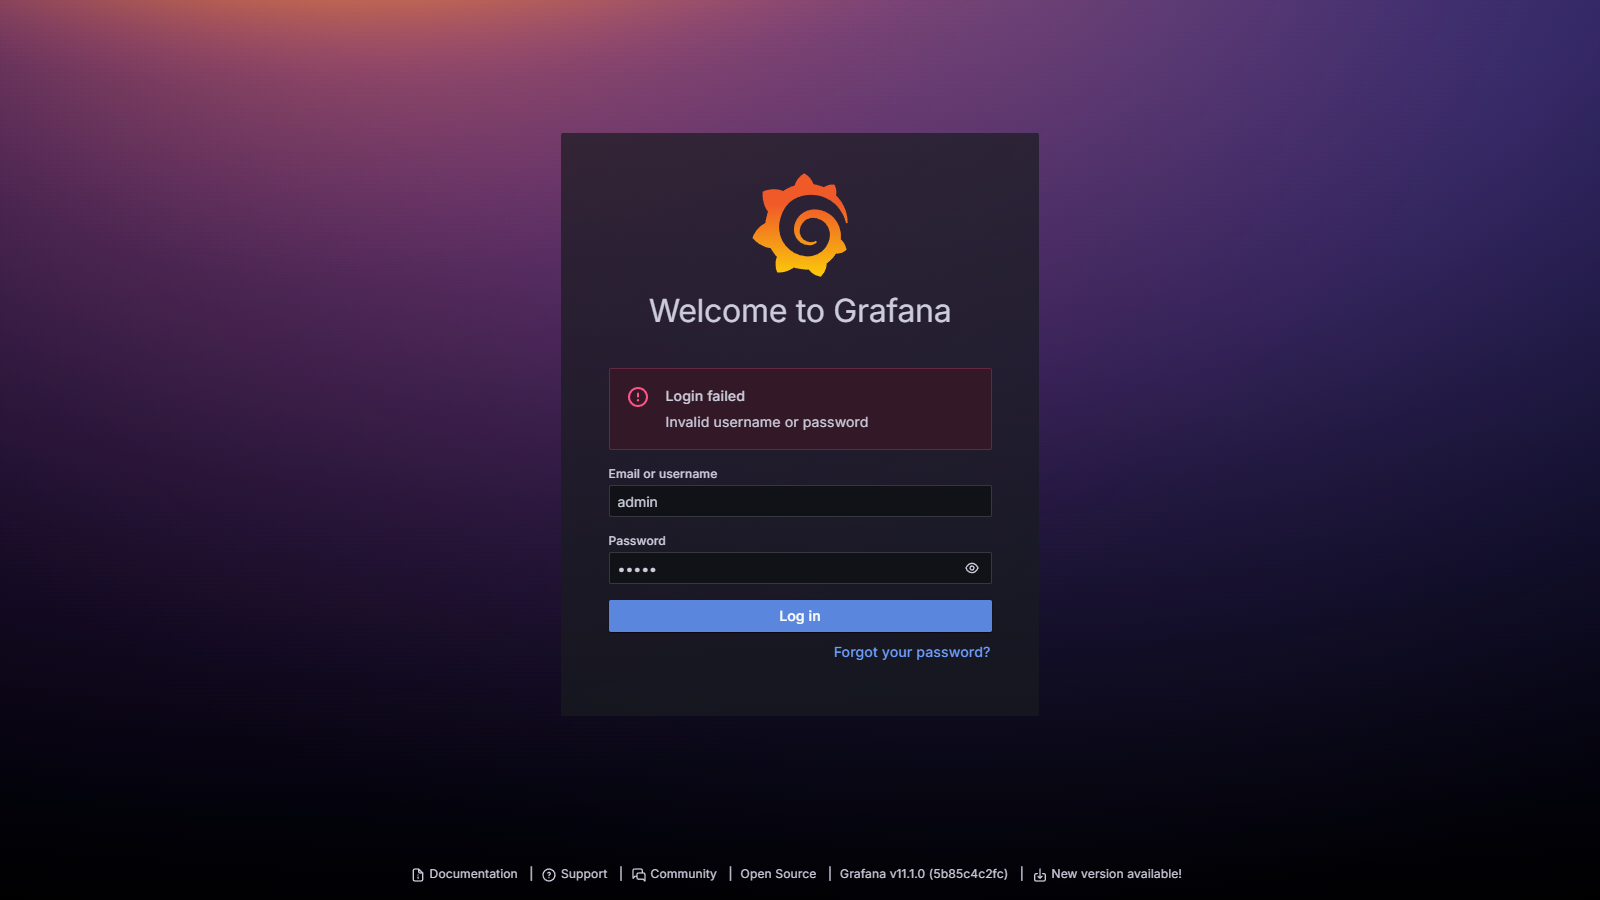
\includegraphics[width=0.9\textwidth,keepaspectratio,trim=0 220 0 180,clip]{gambar/08-login-ditolak.png}
    \caption{Percobaan login dengan kredensial bawaan \texttt{admin/admin} ditolak; password asli tidak dimasukkan.}
    \label{fig:loginditolak}
\end{figure}

\section{Verifikasi End-to-End}
Verifikasi dilakukan terhadap sistem yang benar-benar berjalan. \texttt{docker compose config} valid. Seluruh container utama berstatus \texttt{Up} dan backend \texttt{healthy}. \texttt{promtool check config} serta \texttt{promtool check rules} lulus. Keempat job pada \texttt{/api/v1/targets} berstatus \texttt{up}; jumlah endpoint yang UP adalah lima karena job container memiliki dua target. Semua kueri panel dikembalikan dengan status \texttt{success} dan jumlah series yang tidak nol. Endpoint \texttt{/api/health} Grafana mengembalikan \texttt{database: ok} dan versi 11.1.0. Berkas \texttt{git ls-files} tidak memuat \texttt{.env}, \texttt{opencode.json}, maupun isi folder Playwright.

\chapter{Kesimpulan}
\begin{enumerate}[leftmargin=*]
    \item Stack monitoring berhasil dijalankan dalam satu project Compose bersama aplikasi. Versi image terkunci, volume data tersedia, dan seluruh target pada halaman \texttt{/targets} berstatus \texttt{UP}.
    \item Dashboard Grafana berisi lima panel yang menjawab pertanyaan tentang aplikasi ini, lengkap dengan satuan, ambang, dan deskripsi. Panel status, rasio gagal, laju permintaan, CPU, dan memori semuanya menampilkan data nyata.
    \item Aturan alarm \texttt{LayananMati} terbukti berubah dari \emph{inactive} menjadi \emph{FIRING} setelah backend dihentikan. Alarm berbunyi 92 detik setelah container berhenti dan kembali normal setelah layanan dinyalakan.
    \item Keamanan dasar diterapkan melalui password acak dari \texttt{.env}, penolakan \texttt{admin/admin}, pembatasan port ke loopback, dan pemisahan rahasia dari repositori.
    \item Kendala cAdvisor pada Docker Desktop diselesaikan dengan exporter statistik Docker yang membaca API resmi, tanpa mengubah logika bisnis aplikasi. Kendala tersebut dicatat secara terbuka agar hasil dapat direproduksi.
\end{enumerate}

\section{Tautan Repository}
Repositori tugas tersedia pada alamat berikut:

\begin{center}
\url{https://github.com/brilianfatihwicaksono2005-code/uts-kepkel-2026-brilian/tree/feat/monitoring-p11}
\end{center}

Berkas penting:
\begin{itemize}[leftmargin=*]
    \item \texttt{compose.monitoring.yaml}
    \item \texttt{monitoring/prometheus.yml}
    \item \texttt{monitoring/alerts.yml}
    \item \texttt{monitoring/grafana/provisioning/}
    \item \texttt{backend/app/Http/Middleware/RecordHttpMetrics.php}
    \item \texttt{laporan/main.tex}
\end{itemize}

\chapter{Daftar Pustaka}
\begin{enumerate}[leftmargin=*]
    \item Tim Pengampu Konstruksi dan Evolusi Perangkat Lunak. \emph{Slide Pertemuan 11: Monitoring dan Observability}. 2026.
    \item Prometheus Authors. \emph{Prometheus Documentation}. \url{https://prometheus.io/docs/}.
    \item Grafana Labs. \emph{Grafana Documentation}. \url{https://grafana.com/docs/}.
    \item Prometheus Authors. \emph{PromQL Basics and Cheat Sheet}. \url{https://prometheus.io/docs/prometheus/latest/querying/basics/}.
\end{enumerate}

\end{document}
